\batchmode
\documentclass[a4paper,10pt]{article}
\usepackage{graphicx}
\usepackage{color}
\usepackage{hyperref}
\usepackage{nameref}
\usepackage{fancyvrb}
\hypersetup{urlcolor=cyan, colorlinks=true, linkcolor=blue}
\usepackage{float}

\textheight=25.5cm
\textwidth=17.5cm
\voffset=0.cm
\hoffset=-0.0cm
\oddsidemargin -1cm
\evensidemargin -1cm
\topmargin -2cm
\baselineskip=0.900cm
\setlength{\parindent}{0in}

\graphicspath{{../figures/}}

\newcommand{\ttt}[1]{\texttt{#1}}
\newcommand{\cl}[1]{\textcolor{magenta}{#1}}

\title{LSS: Summary}
\author{Humna Awan, Eric Gawiser}
\date{\today}

\begin{document}
\maketitle
%%%%%%%%%%%%%%%%%%%%%%%%%%%%%%%%%%%%%%%%%%%%%%%%%%%%%%%%%%%
\section*{Summary: Metrics' Interplay}

Large scale structure studies require some important features: survey uniformity over an area that maximizes the usable survey footprint with deep photometric data. To check the survey uniformity, we consider the \nameref{translational dithers} Metric which illustrates the need for large translational dithers. Using the translationally dithered survey, we then use the \nameref{area} metric to define an extragalactic footprint that will give us the galaxy samples we need for our science. We then consider the \nameref{median depth} and \nameref{depth std} Metrics to asses the survey depth and survey uniformity in our footprint. These feed into \nameref{OS systematics} Metric which allows us to assess the impacts of the artifacts that are induced by the observing strategy. \\

Also, in order to maximize the usability of WFD for extragalactic science, we propose a reconfigured WFD footprint, avoiding the high-extinction regions in the sky but still covering the nominal 18,000 deg$^2$. In order to ensure that \nameref{median visits} Metric results are agreeable in this proposed footprint, we have requested an \ttt{OpSim} to get a better sense of coverage we can expect. \\

Furthermore, in order to minimize systematics, we consider the \nameref{rotational dithers} Metric for rotational uniformity and \nameref{4MOST+DESI overlap} Metric to ensure that we optimize the WFD footprint to get the spectroscopic sample we need for our photo-z calibrations. Finally, we consider the \nameref{seeing} Metric in order asses the impacts of variations in seeing as it impacts the size and depth of the sample we can expect to see.

%%%%%%%%%%%%%%%%%%%%%%%%%%%%%%%%%%%%%%%%%%%%%%%%%%%%%%%%%%%
\newpage
\section*{Median Number of Visits Per Field (After Y10)\label{median visits}}
This metric ensures that we are meeting the LSST SRD requirement that the median number of WFD visits per field after Y10 is at least 825.

\begin{minipage}{\columnwidth}
\vspace*{2em}
\centering
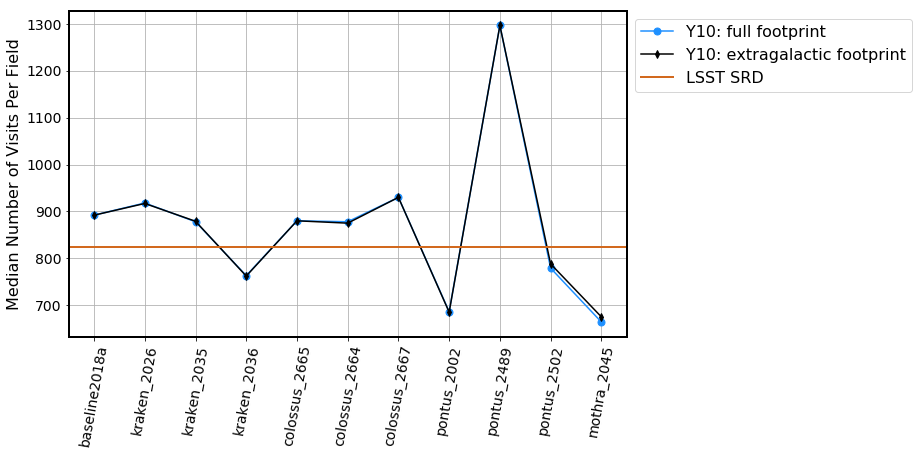
\includegraphics[width=.9\columnwidth]{lss_compare_median_nvisits_11dbs.png}
\vspace*{2em}
\end{minipage}

\cl{Will add the rest of the cadences (i.e., the \ttt{alt\_sched} and \ttt{FBS} outputs) but need to create a \ttt{Stacker} for \ttt{fieldIDs} since the new schedulers don't have \ttt{fieldIDs} associated with visits.}


%%%%%%%%%%%%%%%%%%%%%%%%%%%%%%%%%%%%%%%%%%%%%%%%%%%%%%%%%%%
\newpage
\section*{Rotational Uniformity\label{rotational dithers}}
This metric looks at the distributions of \ttt{rotTelPos} and \ttt{rotSkyPos} for different fields as we'd like them to be uniform. The nominal pointings leads a pile-up in \ttt{rotTelPos} distribution at -90 and 0 degrees. We see that rotational dithers help achieve more uniform distributions for both rotational angles.

\begin{minipage}{\columnwidth}
\vspace*{2em}
\centering
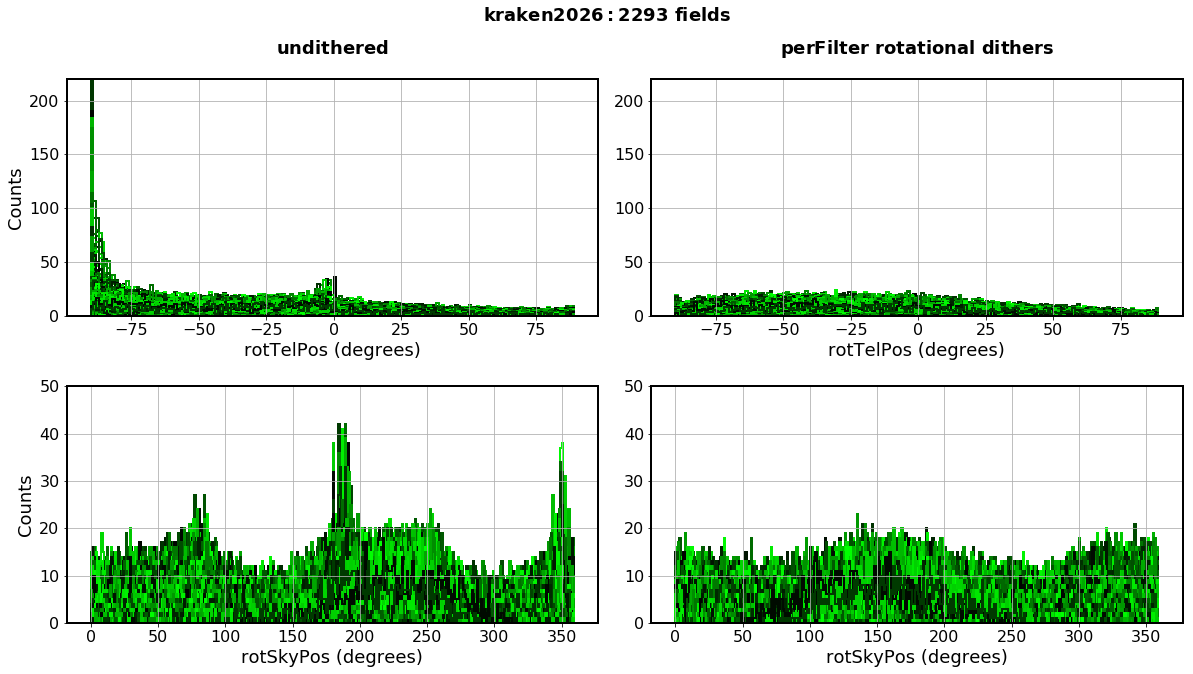
\includegraphics[width=\columnwidth]{lss_compare_rot_angles_kraken_2026_perfield_nodith_wdith.png}
\vspace*{2em}
\end{minipage}
The plot here shows the distributions for WFD visits for \ttt{kraken\_2026}; similar plots for the \ttt{OpSim} dbs can be found \href{https://github.com/LSSTDESC/ObsStrat/blob/issue/3/desc-dithers/code/descDithers/compare_rot_distributions_perfield.ipynb}{here}. A similar analysis can be done for DDF ones.

\cl{The right column will be updated once we have rotational dithers such that we do not dither in between visit pairs. Also, the outputs from new schedulers need to be added but we need a Stacker for addiing \ttt{fields} to these outputs.}

%%%%%%%%%%%%%%%%%%%%%%%%%%%%%%%%%%%%%%%%%%%%%%%%%%%%%%%%%%%
\newpage
\section*{Translational Uniformity\label{translational dithers}}
This metric looks at the need for (large) translational dithers. An undithered survey not only leads to survey non-uniformity but also a comparatively shallower survey. We showed in Awan+16 that translational dithers help with both issues.

\begin{minipage}{\columnwidth}
\vspace*{2em}
\centering
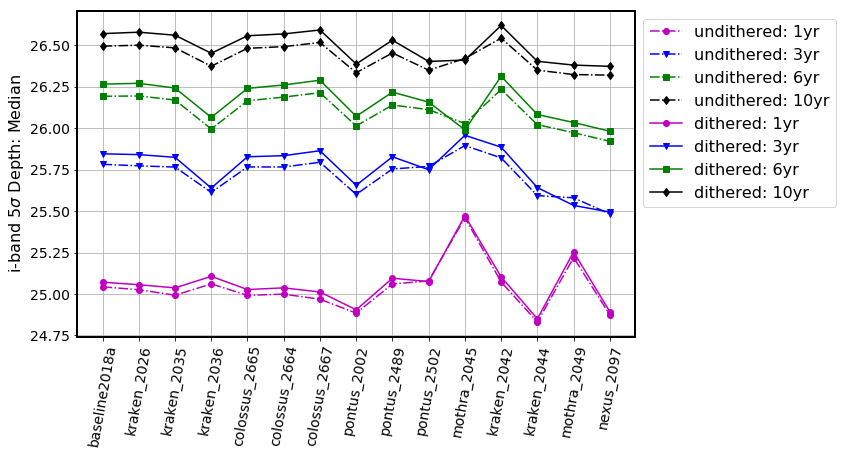
\includegraphics[width=.75\columnwidth]{lss_compare_depth_median_15dbs_undith.png}
\vspace*{2em}
\end{minipage}

\begin{minipage}{\columnwidth}
\vspace*{2em}
\centering
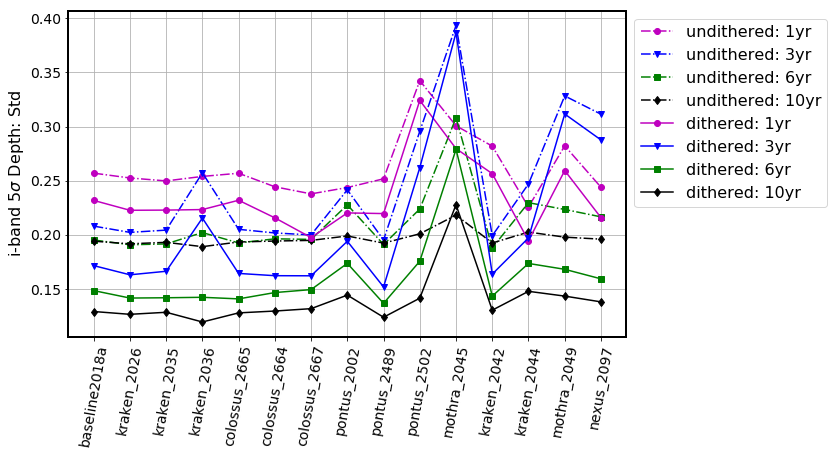
\includegraphics[width=.75\columnwidth]{lss_compare_depth_std_15dbs_undith.png}
\vspace*{2em}
\end{minipage}

Here, the dithered survey implemented per night, random translational dithers, as large as the LSST FOV. Also, the depth statistics are for the extragalactic WFD footprint.

%%%%%%%%%%%%%%%%%%%%%%%%%%%%%%%%%%%%%%%%%%%%%%%%%%%%%%%%%%%
\newpage
\section*{Extragalactic Footprint\label{area}}
This metric looks at the usable WFD area for extragalactic science, which we achieve by implementing an extinction cut and a depth cut on the coadded depth footprint.  Specifically, we retain only the area with E(B-V)$<$0.2 with limiting $i$-band coadded 5$\sigma$ depth of 24.5 for Y1, 25.0 for Y3, 25.5 for Y6, and 26.0 for Y10.

\begin{minipage}{\columnwidth}
\vspace*{2em}
\centering
 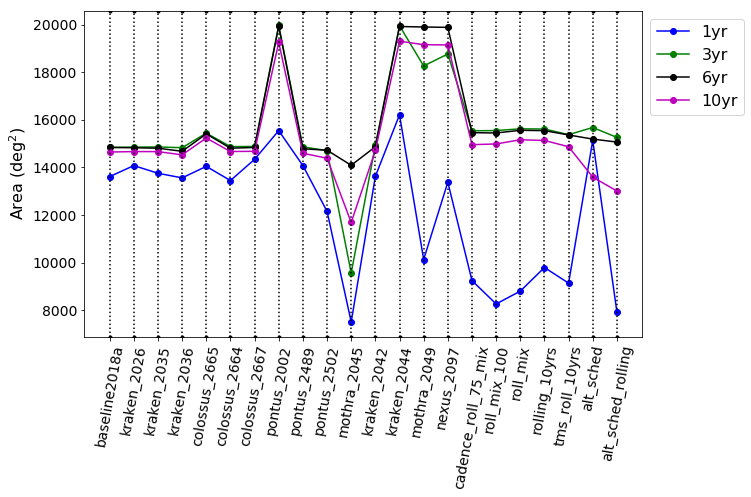
\includegraphics[width=.75\columnwidth]{lss_compare_area_22dbs.png}
\vspace*{2em}
\end{minipage}

\cl{This figure will be updated once we cater our depth cuts to each cadence}.

%%%%%%%%%%%%%%%%%%%%%%%%%%%%%%%%%%%%%%%%%%%%%%%%%%%%%%%%%%%
\newpage
\section*{Median Depth in the Extragalactic Footprint\label{median depth}}
This metric looks at the median depth in the extragalactic footprint. We would like to go deeper to probe fainter galaxy samples to get better constraining power. Here, we look at the $i$-band coadded 5$\sigma$ depth after Y1, 3, 6, 10.

\begin{minipage}{\columnwidth}
\vspace*{2em}
\centering
 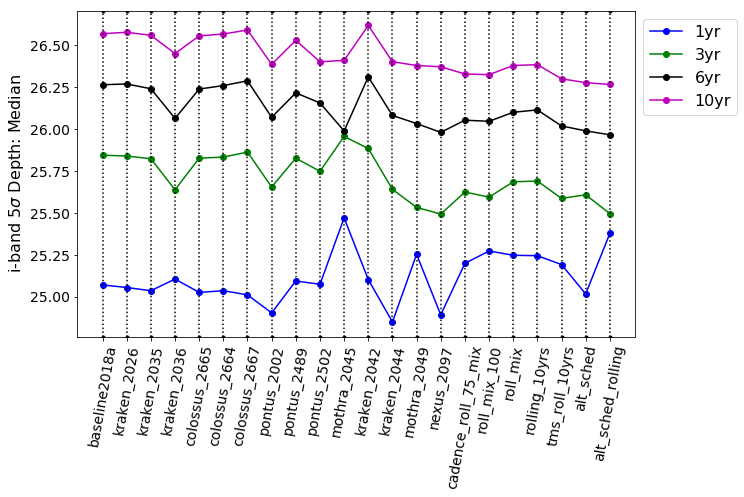
\includegraphics[width=.75\columnwidth]{lss_compare_depth_median_22dbs.png}
\vspace*{2em}
\end{minipage}

\cl{This figure will be updated once we cater our depth cuts to each cadence}.

%%%%%%%%%%%%%%%%%%%%%%%%%%%%%%%%%%%%%%%%%%%%%%%%%%%%%%%%%%%
\newpage
\section*{Depth Uniformity in the Extragalactic Footprint\label{depth std}}
This metric looks at the depth uniformity in the extragalactic footprint. Here, we model this as the standard deviation in the $i$-band coadded 5$\sigma$ depth in the extragalactic footprint.  We would like to minimize non-uniformity to minimize window function uncertainties. 

\begin{minipage}{\columnwidth}
\vspace*{2em}
\centering
 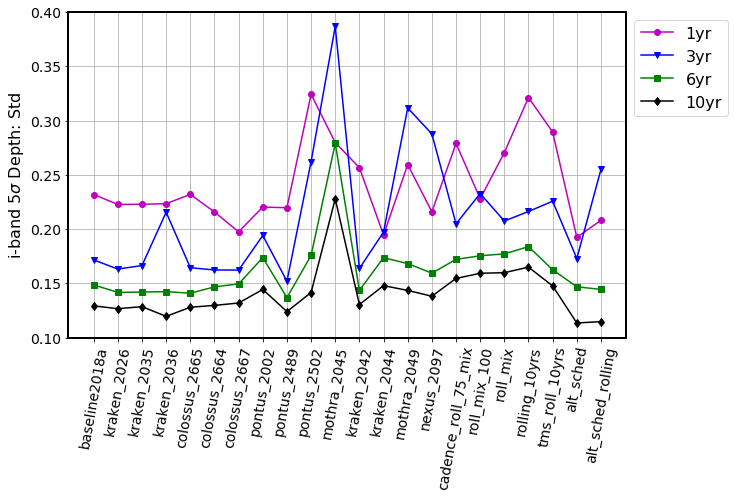
\includegraphics[width=.75\columnwidth]{lss_compare_depth_std_22dbs.png}
\vspace*{2em}
\end{minipage}

\cl{This figure will be updated once we cater our depth cuts to each cadence}.

%%%%%%%%%%%%%%%%%%%%%%%%%%%%%%%%%%%%%%%%%%%%%%%%%%%%%%%%%%%
\newpage 
\section*{Impacts of Artificial Structure on LSS studies\label{OS systematics}}
This metric looks at the effectiveness of each cadence in minimizing the uncertainties in the artificial structure that is induced by the observing strategy. It implements a modified version of the FoM in Equation 9.4 in the LSST Observing Strategy Community White Paper (COSEP). Specifically, we have:
\begin{equation}
	\rm{FoM} \equ iv \sqrt{
			\frac{
				\sum\limits_\ell{ \left({\sqrt{ \frac{2}{f_{\rm{sky, max}} (2\ell + 1)} }
									C_{\ell, \rm{LSS, \clB{Y10}}}} \right)
				}^2
				}{
				\sum\limits_\ell \left[{\left( { \sqrt{\frac{2}{f_{\rm{sky}} (2\ell + 1)}}
									\left\{{C_{\ell, \rm{LSS}} + \frac{1}{\bar{\eta}}} \right\}  } \right ) ^2
									+ \sigma_{C_{\ell,\rm{OS}}}^2  }\right]
				}
			}
\label{eq: LSS FoM COSEP modified}
\end{equation}
where the power spectrum in the numerator differs from that in COSEP as we now use the Y10 gold sample power spectrum to compare the uncertainty acheived with Y10 target sample.\\

For $f_{\rm{fsky, max}}$, we use the Y10 sky coverage with \ttt{baseline2018a} achieved when using random per night dithers; the Y10 footprint is extinction limited (E(B-V)$<$0.2) and depth limited ($i>25.3$ where $i$-band depth is the 5$\sigma$ coadded depth) to achieve the target Y10 gold sample of galaxies.

\begin{minipage}{\columnwidth}
\vspace*{2em}
\centering
 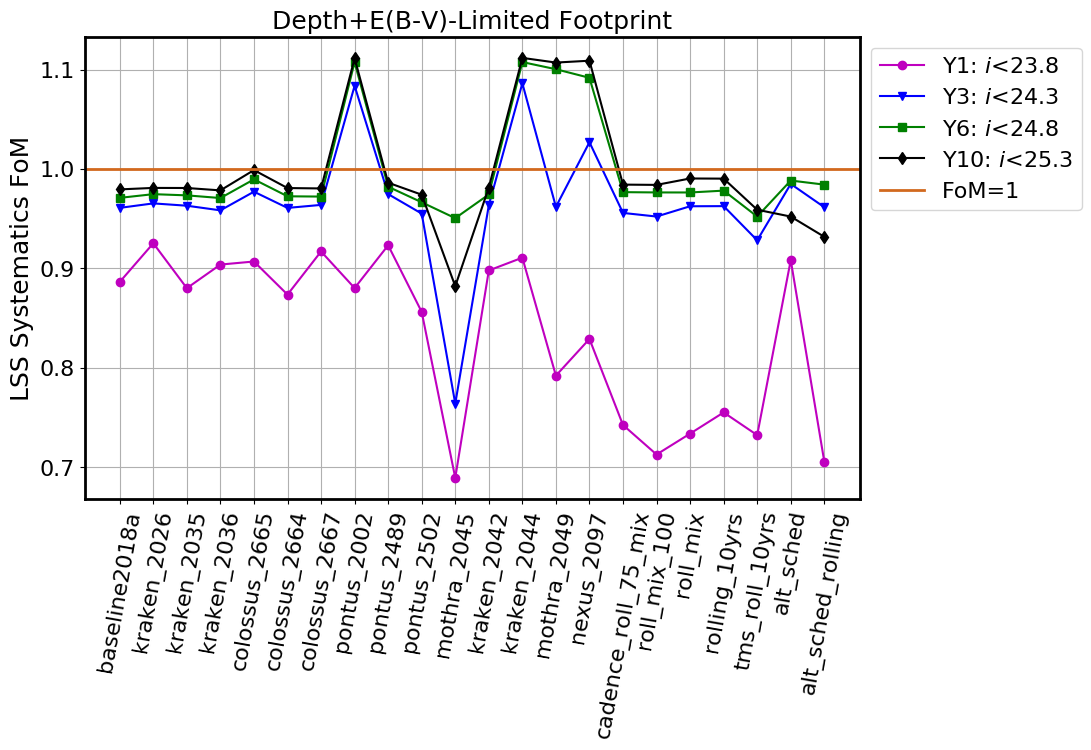
\includegraphics[width=.75\columnwidth]{lss_compare_foms_egfootprint_22dbs_2018-11-24data_srdcuts_noisefom.png}
\vspace*{2em}
\end{minipage}
This plot shows the FoM (Equation~\ref{eq:  LSS FoM COSEP modified}) for different dbs for different years. Note that the depth cuts in the legend are on the extended source coadded depth and (roughly) correspond to the point-source coadded depths in \nameref{area}. We'd like to maximize this FoM as much as possible.

%%%%%%%%%%%%%%%%%%%%%%%%%%%%%%%%%%%%%%%%%%%%%%%%%%%%%%%%%%%
\newpage
\section*{4MOST/DESI Overlap\label{4MOST+DESI overlap}}
This metric looks at the overlap between LSST (extragalactic) footprint and spectroscopic surveys like 4MOST and DESI as we would like the footprint to overlap with either 4MOST or DESI (not necessarily both but potentially a preference for DESI vs 4MOST) for calibrating our photo-$z$s.

\begin{minipage}{\columnwidth}
\vspace*{2em}
\centering
 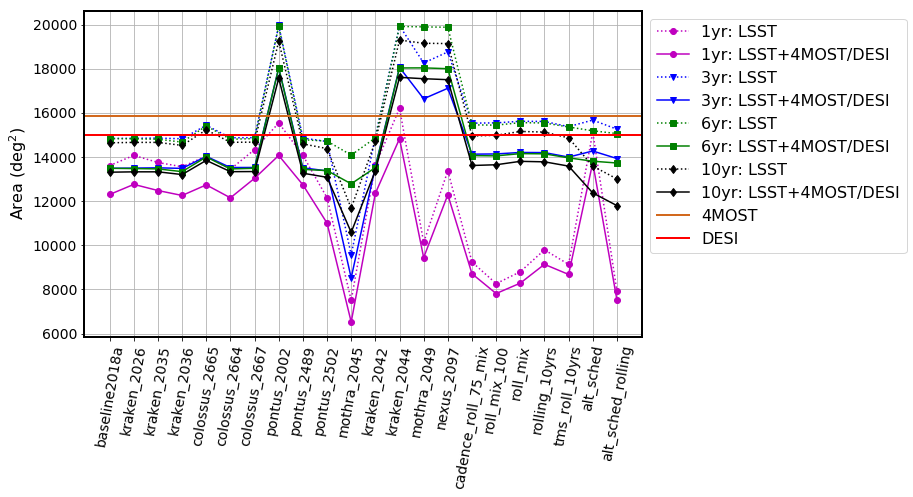
\includegraphics[width=.8\columnwidth]{lss_compare_LSST+4MOSTorDESI_overlap_22dbs.png}
\vspace*{2em}
\end{minipage}

%%%%%%%%%%%%%%%%%%%%%%%%%%%%%%%%%%%%%%%%%%%%%%%%%%%%%%%%%%%
\newpage
\section*{Impacts of Seeing\label{seeing}}
This metric looks at the impacts of seasonal variations in seeing, as implemented by Eric Nielson. It is critical to get realistic seeing implemented in our simulated cadences as ignoring seeing variations leads to inaccurate calculation of the 5$\sigma$ point-source depth which impacts all derived quantities, e.g. the coadded 5$\sigma$ depth.

\begin{minipage}{\columnwidth}
\centering
\vspace*{2em}
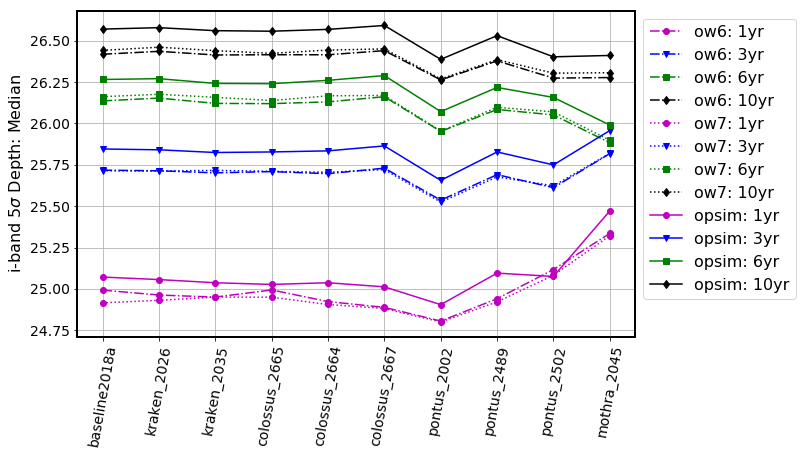
\includegraphics[width=.75\columnwidth]{lss_compare_depth_median_10dbs_ow6_ow7_opsim.png}
\vspace*{2em}
\end{minipage}

Here, \ttt{ow6} and \ttt{ow7} identify two different outputs from \ttt{owsee}, using data from different but overlapping years in Pachon.


\end{document}
